
\chapter{Discretización de segundo orden de la ecuación de Burgers}\label{articuloburger}

En este capítulo presentamos y aplicamos una alternativa a la discretización implícita tradicional llamada método de Crank-Nicholson, el cual aplicaremos directamente sobre la ecuación no lineal de Burgers (\ref{BE}). Con tal discretización obtendremos un sistema de ecuaciones no lineales (para cada instante) $F(u(x,t_j))=0$, que deberá ser resuelto mediante el uso de método iterativos de punto fijo.
Concretamente usaremos el método clásico de Newton (cuyo orden de convergencia es dos),
\begin{eqnarray} \label{newton}
x^{(k+1)}=x^{(k)}-[F'(x^{(k)})]^{-1}F(x^{(k)}),
\end{eqnarray}
el método de Traub de orden tres (ver \cite{TR})
\begin{eqnarray} \label{traub}
y^{(k)}=x^{(k)}-[F'(x^{(k)})]^{-1}F(x^{(k)}), \\\nonumber
x^{(k+1)}=y^{(k)}-[F'(x^{(k)})]^{-1}F(y^{(k)})
\end{eqnarray}
y el método denotado como M5 (ver \cite{ACT}), de orden de convergencia cinco, cuya expresión iterativa es,
\begin{eqnarray} \label{m5}
y^{(k)}&=&x^{(k)}-[F'(x^{(k)})]^{-1}F(x^{(k)}), \\ \nonumber
z^{(k)}&=&y^{(k)}-5[F'(x^{(k)})]^{-1}F(y^{(k)}), \\
x^{(k+1)}&=&z^{(k)}-\frac{1}{5}
[F'(x^{(k)})]^{-1}[-16F(y^{(k)})+F(z^{(k)})].\nonumber
\end{eqnarray}

La estabilidad del método es analizada numéricamente, comprobando que se trata de un método incondicionalmente estable. El método de Crank-Nicholson presentado tiene una precisión de segundo orden tanto en el espacio como en el tiempo. El método será puesto a prueba mediante el uso de distintos valores de $\varepsilon$ y distintas condiciones iniciales con el objetivo de analizar su estabilidad y consistencia; para llevar esto a cabo, la solución obtenida a partir de los métodos iterativos es comparada entre ellos así como con la solución exacta. Estos resultados, así como sus interesantes conclusiones, fueron presentados en la \textit{``16th Edition of the	Mathematical Modelling Conference Series''} y publicados por la revista \textit{Algorithms 8(2015) 224-233} bajo el título \textit{``Numerical Solution of Turbulence Problems by Solving Burgers’ Equation''} (véase \cite{paperburgers}).

Ahora, consideremos la ecuación en derivadas parciales unidimensional de Burgers (ver \cite{Bateman} y \cite{Burgers}),
\begin{equation}\label{BE}
\frac{\partial u}{\partial t}+u \frac{\partial u}{\partial
	x}=\frac{1}{Re} \frac{\partial^2 u}{\partial^2 x}, \ \ (x,t)\in
\Omega
\end{equation}
donde $\Omega=(a,b)\times(0,T]$. La condición inicial es tal que $u(x,0)=f(x)$, $a<x<b$ y las de contorno son tales que $u(a,t)=g_1(t)$,
$u(b,t)=g_2(t)$, $0\leq t \leq T$; siendo $Re$ el número de Reynolds 
y $f$, $g_1$ y $g_2$ unas funciones dadas suficientemente suaves. Por simplicidad, algunas veces usaremos $\varepsilon$ en vez de $\frac{1}{Re}$.

La ecuación de Burgers es usada para la descripción de problemas de turbulencia, en la teoría de las ondas sísmicas y en procesos estocásticos continuos. Tiene aplicaciones en dinámica de gases, conducción del calor y elasticidad, entre otras.

Este problema muestra una estructura bastante similar a la de las ecuaciones de Navier-Stokes, debido a la forma del término no lineal de convección y la existencia del término correspondiente a la viscosidad. Así pues, éste puede ser considerado como una forma simplificada de la ecuación de Navier-Stokes. En estos últimos años, diversos investigadores han usado distintos métodos numéricos, especialmente basados en diferencias finitas, técnicas de frontera de elementos finitos y métodos variacionales, con el objetivo de resolver este problema (ver, por ejemplo, \cite{KA,HSH,WT} y las referencias que se citan en su interior).

Además, la ecuación no lineal de Burgers \eqref{BE} es una de las pocas ecuaciones en derivadas parciales no lineal cuya solución puede ser obtenida analíticamente de forma exacta para una función inicial arbitraria $f(x)$. La denominada transformación de Hopf-Cole \cite{H-C}
\begin{equation}\label{transformation}
u(x,t)=-\left( \frac{2}{Re} \right) \frac{\phi_x(x,t)}{\phi(x,t)},
\end{equation}
facilita dicha resolución, siendo $\phi$ la solución a la ecuación lineal de difusión
\begin{equation}\label{ecdiffusion}
\frac{\partial \phi(x,t)}{\partial t}=\frac{1}{Re} \frac{\partial^2
	u}{\partial^2 x}.
\end{equation}
Siendo $u$ la solución de la ecuación de Burgers (\ref{BE}). Esta transformación nos permite obtener los valores exactos de $u(x,t)$ porque la ecuación (\ref{ecdiffusion}) tiene una solución en series de Fourier, sin embargo, su coste computacional es muy elevado y por eso nosotros sólo la usamos para comparar la precisión de nuestros resultados (como veremos un poco más adelante, las integrales de los coeficientes de Fourier deben ser calculadas). Como podemos ver en \cite{KA}, algunos investigadores han aprovechado esta transformación y han aplicado el método de Crank-Nicholson sobre la ecuación lineal (\ref{ecdiffusion}) con el objetivo de obtener en primer lugar los valores de $\phi(x,t)$ y posteriormente los de $u(x,t)$. Otros autores han usado el método implícito, donde $\frac{\partial u}{\partial t}$ es aproximado por diferencias finitas regresivas, sin embargo debido a que su error de truncamiento es de orden uno, la precisión de los resultados decrece.

La forma más fácil de discretizar un problema de ecuaciones en derivadas parciales (como el que tenemos en la ecuación (\ref{BE})) consiste en reducir el dominio continuo a un número finito de puntos equiespaciados $(x_i,t_j)$, localizados en los nodos de un mallado rectangular uniforme. Así pues, ahora las derivadas parciales de $u$ pueden ser aproximadas por los siguientes cocientes de diferencias 
\begin{equation} \label{forward}
\frac{\partial u(x_i,t_j)}{\partial x}\approx\frac{u_{i+1,j}-u_{i,j}}{h}, \qquad\frac{\partial u(x_i,t_j)}{\partial t}\approx\frac{u_{i,j+1}-u_{i,j}}{k}
\end{equation}
las cuales son llamadas diferencias progresivas, y tienen un error de truncamiento de orden 1. Las derivadas parciales de $u$ también pueden ser obtenidas a partir de
\begin{equation} \label{backward}
\frac{\partial u(x_i,t_j)}{\partial x}\approx\frac{u_{i,j}-u_{i-1,j}}{h}, \qquad\frac{\partial u(x_i,t_j)}{\partial t}\approx\frac{u_{i,j}-u_{i,j-1}}{k},
\end{equation}
las cuales son llamadas diferencias regresivas, y también tienen un error de truncamiento de orden 1. Finalmente, las derivadas parciales de $u$ también pueden ser obtenidas a partir de
\begin{equation} \label{central}
\frac{\partial u(x_i,t_j)}{\partial x}\approx\frac{u_{i+1,j}-u_{i-1,j}}{2h}, \qquad\frac{\partial u(x_i,t_j)}{\partial t}\approx\frac{u_{i,j+1}-u_{i,j-1}}{2k},
\end{equation}
\begin{equation} \label{centralsecond}
\frac{\partial^2 u(x_i,t_j)}{\partial x^2}\approx\frac{u_{i+1,j}-2u_{i,j}+u_{i-1,j}}{h^2}, \qquad\frac{\partial^2 u(x_i,t_j)}{\partial t^2}\approx\frac{u_{i,j+1}-2u_{i,j}+u_{i,j-1}}{k^2},
\end{equation}
las cuales son llamadas diferencias centrales, y tienen un error de truncamiento de orden 2. En estas expresiones, $u_{i,j}$ denota el valor aproximado de la función incógnita $u$ en $(x_i,t_j)$, $h=\frac{b-a}{n}$, y $k=\frac{T-0}{m}$ son, respectivamente, el paso en el espacio y el tiempo del mallado, y $n$ y $m$ son, respectivamente, la cantidad de subintervalos considerados en el dominio del espacio y del tiempo. Así pues, tenemos que $x_{i+1}=x_i+h$ y $t_{j+1}=t_j+k$, donde $i=0,1,...,n-1$ y
$j=0,1,...,m-1$.

Apliquemos ahora el esquema en diferencias de Crank-Nicholson, el cual consiste en discretizar la ecuación (\ref{BE}) en dos instantes de tiempo consecutivos y promediarlos. En el primer instante $t_j$, aproximamos $\frac{\partial u}{\partial t}$ por las diferencias progresivas descritas en la ecuación (\ref{forward}), y en el segundo instante $t_{j+1}$, lo hacemos por las regresivas. En ambos instantes aproximamos $\frac{\partial u}{\partial x}$ y $\frac{\partial^2u}{\partial x^2}$  por las diferencias centrales (descritas en las ecuaciones (\ref{central}) y (\ref{centralsecond}), respectivamente). Por medio de este procedimiento obtenemos, para el primer instante,
\begin{equation} \label{firstinstant}
\frac{u_{i,j+1}-u_{i,j}}{k}-\varepsilon\frac{u_{i+1,j}-2u_{i,j}+u_{i-1,j}}{h^2}+u_{i,j}\frac{u_{i+1,j}-u_{i-1,j}}{2h}=0
\end{equation}
y para el segundo,
\begin{equation} \label{secondinstant}
\frac{u_{i,j+1}-u_{i,j}}{k}-\varepsilon\frac{u_{i+1,j+1}-2u_{i,j+1}+u_{i-1,j+1}}{h^2}+u_{i,j+1}\frac{u_{i+1,j+1}-u_{i-1,j+1}}{2h}=0.
\end{equation}
Después de promediar ambas expresiones, resulta
\begin{eqnarray} \label{average}
Bu_{i,j+1}u_{i+1,j+1}-Bu_{i,j+1}u_{i-1,j+1}-Cu_{i+1,j+1}+2Cu_{i,j+1}-Cu_{i-1,j+1}+Au_{i,j+1}=\\\nonumber Cu_{i+1,j}+(A-2C)u_{i,j}+Cu_{i-1,j}+Bu_{i,j}u_{i+1,j}-Bu_{i,j}u_{i-1,j}
\end{eqnarray}
donde $A=\frac{1}{k}$, $B=\frac{1}{4h}$,
$C=\frac{\varepsilon}{2h^2}$ y el rango de índices es
$i=1,...,n-1$ y $j=0,1,...,m-1$. Esta expresión (la cual tiene un error de truncamiento de orden 2) resulta en $m$ sistemas no lineales de $n-1$ incógnitas y $n-1$ ecuaciones. Cada uno de estos sistemas aparece tras considerar que ya conocemos de antemano el valor de $u_{0,j}$ y	$u_{n,j}$, $\forall j$ (de las condiciones de contorno) y $u_{i,0}$,
$\forall i$ de la condición inicial. Nótese que los valores correspondientes al subíndice $j$ han sido calculados en el sistema previo al actual, y que las únicas incógnitas serán aquellas con el subíndice $j+1$.

\section{Resultados numéricos}
Comparemos pues, nuestros resultados con los de la solución exacta, la cual puede ser obtenida mendiante la transformación de Hopf-Cole mencionada en las ecuaciones 	(\ref{transformation}) y (\ref{ecdiffusion}). Para ello, primero calculamos
\[
\phi(x,t)=A_0+\sum\limits_{p=1}^\infty
A_pe^{-p^2\varepsilon\pi^2t}\cos{(p\pi x)}
\]
y posteriormente, a partir de la ecuación (\ref{transformation}), obtenemos
\begin{equation}\label{uanalitica}
u(x,t)=2\pi\varepsilon\frac{\sum_{p=1}^\infty
	A_pe^{-p^2\varepsilon\pi^2t} p\ \ \sin{(p\pi
		x)}}{A_0+\sum_{p=1}^\infty A_pe^{-p^2\varepsilon\pi^2t}\cos{(p\pi
		x)}}
\end{equation}
donde
\[
A_0=\int_{a}^{b} e^{-\frac{1}{2\varepsilon}\int_{a}^{x} u(\xi,0)d\xi} dx,
\]
\[
A_p=2\int_{a}^{b} e^{-\frac{1}{2\varepsilon}\int_{a}^{x}
	u(\xi,0)d\xi} \cos{(p\pi x)}dx, \ \ p=1,2,\ldots
\]
Nuestro objetivo, para poder demostrar la precisión de nuestros resultados, es obtener por lo menos cinco decimales exactos de la solución, y para ello hemos observado que es suficiente con coger tan sólo dos sumandos de la serie de Fourier. Así pues, sólo tenemos que calcular $A_0$, $A_1$ y $A_2$. Dichos coeficientes son calculados en formato \textit{long} mediante la función \textit{int(integrando,limite\_inferior,limite\_superior)} de Matlab.

En los ejemplos mostrados a continuación, consideramos que las condiciones de contorno son cero, así pues \mbox{$g_1(t)=0$} y $g_2(t)=0$, lo que significa que $u_{0,j}=0$ y $u_{n,j}=0$, $\forall j$. En este caso podemos comparar nuestros resultados con la solución exacta, sin embargo nuestro método ha resultado ser incondicionalmente estable, numéricamente hablando, para todas las condiciones de contorno utilizadas. Para la obtención de ambas soluciones, la exacta y la aproximada, se ha usado la versión R2013a de Matlab, con doble precisión. El criterio de parada usado es
$$\|u^{(k+1)}(x,t_j)-u^{(k)}(x,t_j)\|+\|F(u^{(k+1)}(x,t_j))|<10^{-15}$$.
%\vspace{0.5 cm}
\textbf{Ejemplo 1.} Las condiciones iniciales y de contorno de la ecuación de Burgers para este ejemplo son
\[
u(x,0)=\frac{2\varepsilon \beta \pi sin(\pi x)}{\alpha+\beta cos(\pi x)}, \qquad 0\le x\le 2
\]
y $u(0,t)=u(2,t)=0, t\ge 0$ donde $\alpha=5$ y $\beta=4$.
\vspace{0.25 cm}

En las Tablas \ref{compn} a \ref{compe} se muestra, para distintos valores de $n$, $m$
y $\varepsilon$, el número medio de iteraciones requeridas al usar los métodos de Newton, Traub y M5. También mostramos el error máximo, EM, que se obtiene para cada valor de $x_i$ y $t_j$, donde $i=0,1,...,n-1$ y $j=0,1,...,m-1$. La aproximación inicial de cada sistema no lineal a resolver es la solución del anterior (y para el primer sistema, la aproximación inicial es el valor exacto de la condición inicial). A continuación obtenemos la matriz de errores como la diferencia absoluta entre la solución aproximada y la solución exacta en cada nodo, finalmente llamamos el error máximo al mayor elemento de esa matriz. Mientras que otros autores prefieren comparar y dar el valor del error sólo en algunos puntos del mallado, nosotros hemos preferido un criterio más riguroso, éste consiste en comparar todos los valores del error de la matriz de errores y dar el valor del EM, de esta forma nos hacemos una mejor idea sobre cómo de mala es la peor situación posible, y sabemos con toda seguridad que el error del resto de puntos será siempre inferior a este EM; de la otra forma no podemos saber si realmente existe algún otro punto cuyo error sea mayor.

Un resultado interesante se desprende de la matriz de errores cuando el tiempo de observación es suficientemente grande, lo cual se puede conseguir mediante una rápida atenuación (valores grandes de $\varepsilon$) o mediante un largo tiempo de estudio (valores grandes de $T$). Si obtenemos el EM entre todos los valores de $x$ para cada tiempo, observamos que el EM se incrementa muy deprisa al principio pero que una vez se alcanza el máximo, éste empieza a decrecer. Este resultado se puede ver en la Figura \ref{atenuaciones}.

En la Tabla \ref{compn} establecemos el tiempo máximo de estudio, la cantidad de nodos en el tiempo y la constante de Reynolds, como $t_{max}=1$,
$m=100$ y $\varepsilon =\frac{1}{Re}=0.1$, y variamos la cantidad de nodos espaciales. Para cada caso obtenemos el ya mencionado EM y el número medio de iteraciones ($\bar{K}$) requeridas para resolver cada sistema no lineal mediante el uso del método de Newton, Traub y M5. De estos resultados observamos que, en general, cuantos más subintervalos espaciales cojamos (paso espacial más pequeño), menor es el EM.

En la Tabla \ref{compm} repetimos el mismo proceso, pero en este caso fijamos la cantidad de nodos en el espacio y variamos la cantidad de nodos en el tiempo. Así pues, $t_{max}=1$, $n=100$ y $\varepsilon =\frac{1}{Re}=0.1$. Como podemos observar, en un primer momento parece que cuantos más subintervalos en el tiempo cojamos, menor es el EM (de forma similar a como pasó con la Tabla \ref{compn}, donde probamos cantidades distintas de subintervalos en el espacio), sin embargo existe un límite a partir del cual el error empieza a incrementarse de nuevo. Para este caso, el error mínimo es obtenido con $m=20$.

\begin{figure}[h!]
	\centering
	\subfloat[$\varepsilon =1$]{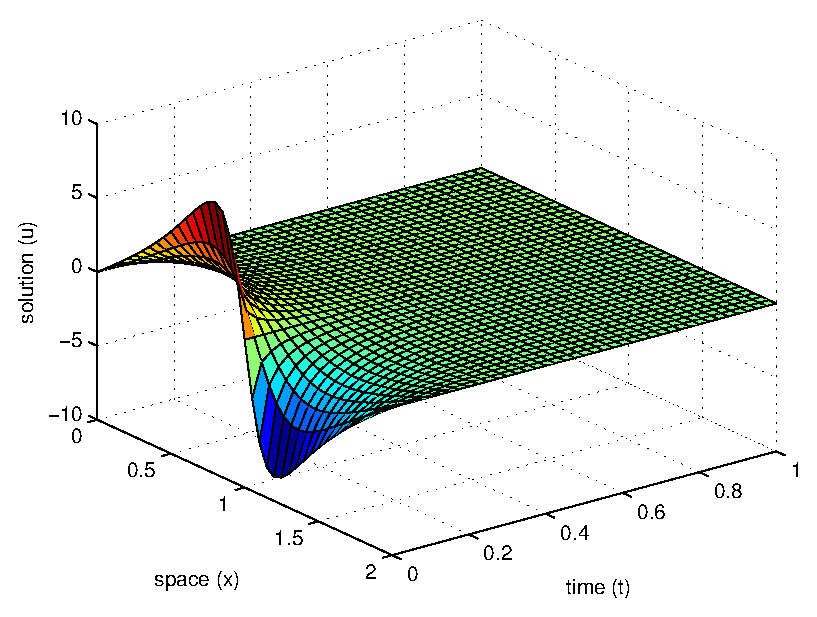
\includegraphics[width=0.33\textwidth]{uepsilon1.eps}} %\hspace{0.5cm}
	\subfloat[$\varepsilon =0.1$]{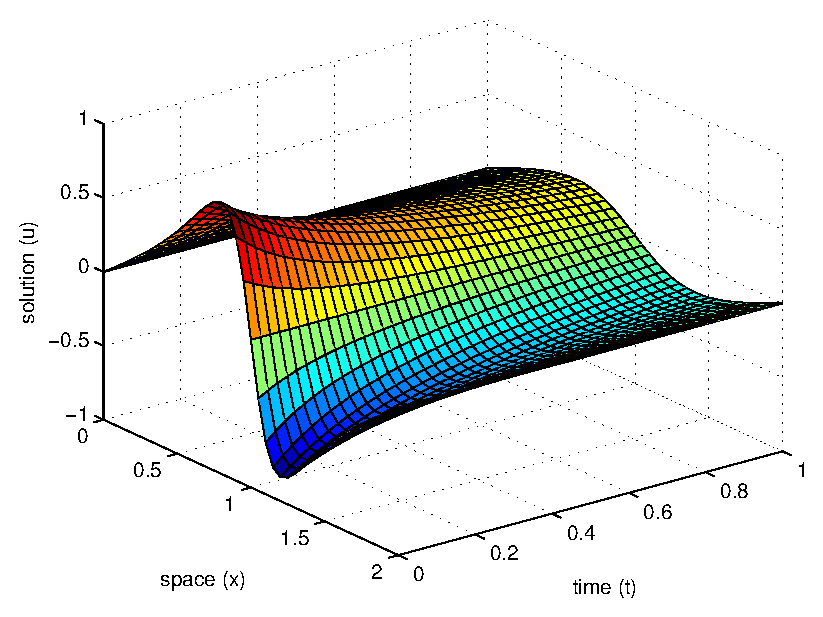
\includegraphics[width=0.33\textwidth]{uepsilon01.eps}} %\hspace{0.5cm}
	\subfloat[$\varepsilon =0.005$]{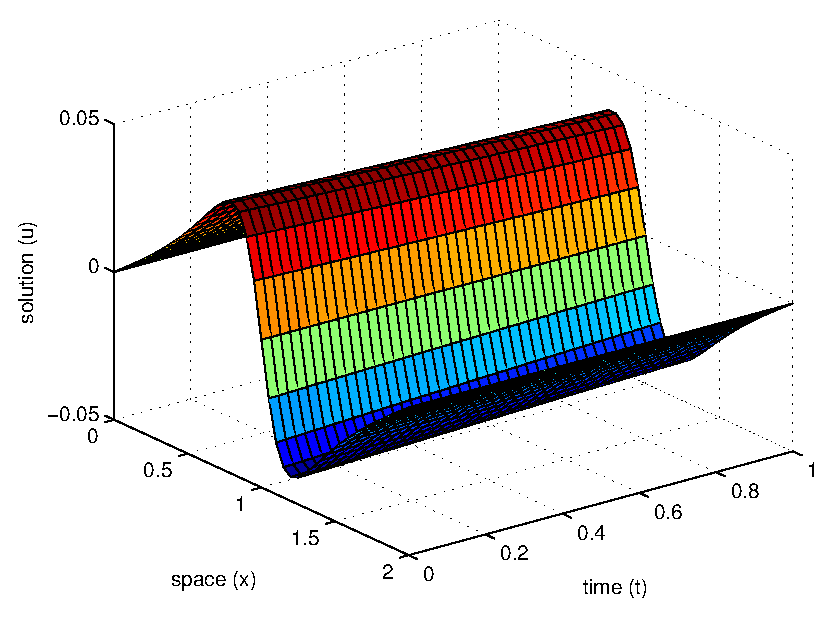
\includegraphics[width=0.33\textwidth]{uepsilon0005.eps}} \\
	\subfloat[$\varepsilon =1$]{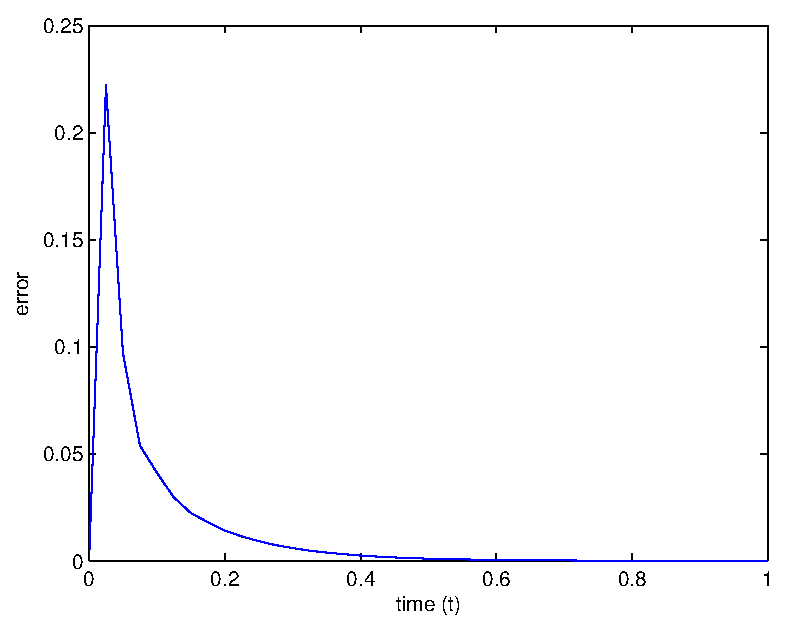
\includegraphics[width=0.33\textwidth]{errorepsilon1.eps}} %\hspace{0.5cm}
	\subfloat[$\varepsilon =0.1$]{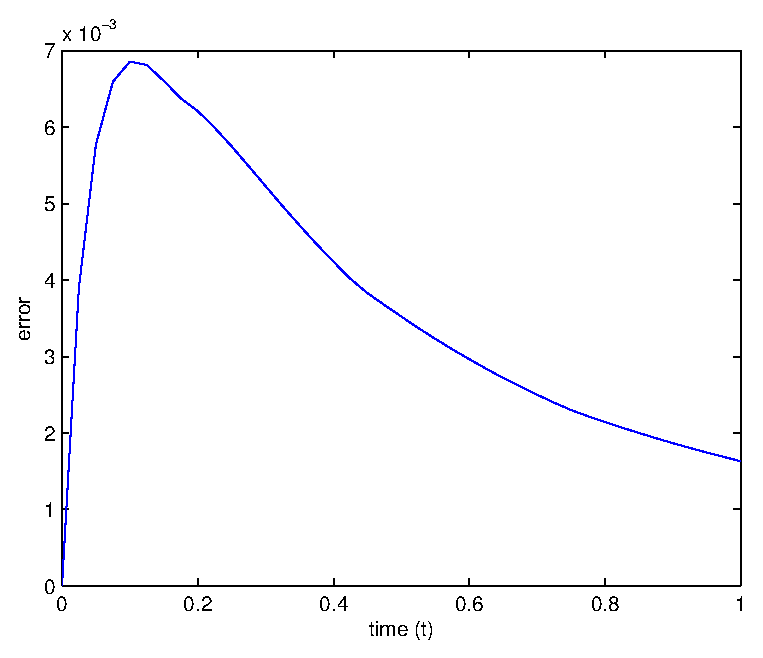
\includegraphics[width=0.33\textwidth]{errorepsilon01.eps}} %\hspace{0.5cm}
	\subfloat[$\varepsilon =0.005$]{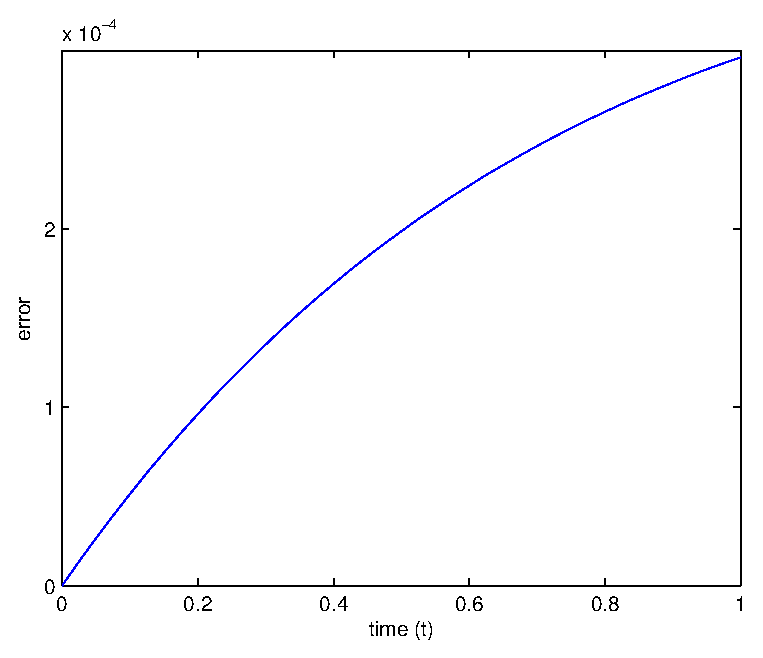
\includegraphics[width=0.33\textwidth]{errorepsilon0005.eps}} \vspace{6pt}
	\caption{Solución aproximada y curva de la progresión del error máximo para distintos tiempos y valores de $\varepsilon$, con \mbox{$n=m=40$} y $t_{max}=1$.}
	\label{atenuaciones}
\end{figure}

%\vspace{-12pt}
\begin{table}[h!]
	\centering
	\small
	\begin{tabular}{cccccc}
		\toprule
		&\boldmath $n=10$ &\boldmath $n=20$ &\boldmath $n=40$ &\boldmath $n=80$ &\boldmath $n=160$ \\ \midrule
		\multicolumn{1}{c}{Error máximo}    & 0.09033    &  0.029932   &  0.0070658   & 0.0017149   &   0.00039376   \\
		\multicolumn{1}{c}{$\bar{K}_N$} &  4   &  4   &   4  &  4   &  4    \\
		\multicolumn{1}{c}{$\bar{K}_T$}  &  3   &   3  &   3  &   3  &   3   \\
		\multicolumn{1}{c}{$\bar{K}_{M5}$}     &  3    &  3   &  3   &  3   &   3   \\ \bottomrule
	\end{tabular}
	\caption{Comparación del EM (error máximo) y las iteraciones por método, para distintas cantidades de subintervalos en el espacio.}\label{compn}
\end{table}

\begin{table}[h!]
	\centering
	\small
	\begin{tabular}{cccccc}
		\toprule
		&\boldmath $m=10$ &\boldmath $m=20$ &\boldmath $m=40$ &\boldmath $m=80$ &\boldmath $m=160$ \\ \midrule
		\multicolumn{1}{c}{Error máximo}    & 0.0043069    &  0.00015291   & 0.00083542   & 0.0010565  & 0.0011128    \\
		\multicolumn{1}{c}{$\bar{K}_{N}$} &  4.4  & 4.15  & 4   &   4 &  4   \\
		\multicolumn{1}{c}{$\bar{K}_{T}$}  &  3.4  &  3.1  &  3  &  3  &  3   \\
		\multicolumn{1}{c}{$\bar{K}_{M5}$}     &  3    &   3   &  3  &  3  &  3   \\ \bottomrule
	\end{tabular}
	\caption{Comparación del EM (error máximo) y las iteraciones por método, para distintas cantidades de subintervalos en el tiempo.}\label{compm}
\end{table}

En la Tabla \ref{compe} repetimos nuevamente el proceso, sin embargo esta vez estudiamos el efecto de escoger un valor pequeño, normal o grande de la constante de Reynolds ($Re$); aunque en verdad usamos $\varepsilon=\frac{1}{Re}$, por simplicidad. Para ello fijamos la cantidad de nodos en el espacio y el tiempo, así como el tiempo máximo de estudio. De esta forma tenemos que $t_{max}=1$,	$n=40$ y $m=40$.

\begin{table}[h!]
	\centering
	\small
	\begin{tabular}{cccccccc}
		\toprule
		&\boldmath $\varepsilon = 1$ &\boldmath $\varepsilon = 0.1$ &\boldmath $\varepsilon = 0.05$ &\boldmath $\varepsilon = 0.03$ &\boldmath $\varepsilon = 0.02$ &\boldmath $\varepsilon = 0.01$ &\boldmath $\varepsilon = 0.005$ \\ \midrule
		\multicolumn{1}{c}{Error máximo}    & 0.22216 & 0.0068572 & 0.0035207 & 0.0021242 & 0.0014188 & 0.000708 & 0.000296 \\
		\multicolumn{1}{c}{$\bar{K}_{N}$} & 3.9 & 4 & 4 & 4 & 4 & 3.85 & 3 \\
		\multicolumn{1}{c}{$\bar{K}_{T}$}  & 3.15 & 3 & 3 & 3 & 3 & 3 & 3 \\
		\multicolumn{1}{c}{$\bar{K}_{M5}$}     & 2.8 & 3 & 3 & 3 & 3 & 3 & 2 \\ \bottomrule
	\end{tabular}
	\caption{Comparación del EM y las iteraciones por método, para distintos valores de $\varepsilon$.}\label{compe}
\end{table}

Es importante recalcar que el valor máximo de $\varepsilon$ que se puede usar para mantener el método funcionando debidamente dependerá de la cantidad de subintervalos que cojamos, esto ocurre debido a que como mayor es la atenuación, más abruptas son las curvas en el eje del tiempo. Para mantener un error pequeño se requiere un mallado más fino, lo cual se puede obtener incrementando la cantidad de subintervalos en el tiempo. En la Tabla \ref{compe} podemos ver numéricamente este fenómeno. Para una rápida atenuación ($\varepsilon = 1$) el error es bastante grande debido a que la curva es muy abrupta (como hemos dicho podríamos reducir el error de este caso tomando más subintervalos en el tiempo), sin embargo cuanto más lenta es la atenuación (valores bajos de $\varepsilon$), más bajo es el EM. Si seguimos cogiendo valores bajos de atenuación ($\varepsilon$ pequeña), el pico de la curva característica del EM no será alcanzado, y en consecuencia el EM será incluso más pequeño (para este ejemplo ésto sucede para $\varepsilon = 0.01$ e incluso más para $\varepsilon = 0.005$). Véase la Figura \ref{atenuaciones} para una mejor comprensión de estas diferentes situaciones.

De las Tablas \ref{compn} a la \ref{compe} se desprenden algunas conclusiones: usar un método de orden más alto (como el M5) no representa una mayor ventaja comparado con un método típico de orden tres (como el de Traub), sin embargo sí existe una diferencia significante entre usar un método de tercer orden y uno típico de segundo (como el de Newton). Cuantos más subintervalos en el espacio cojamos, menor es el EM; sin embargo, esto no ocurre con la cantidad de subintervalos en el tiempo, lo cual significa que hay una cantidad óptima de subintervalos en el tiempo que reduce el EM hasta su mínimo, pero pasado éste el error empieza a incrementarse de nuevo, y el incremento del coste computacional (debido al incremento de operaciones en coma flotante, tiempo de ejecución, etc.) de tener que resolver tantos sistemas no conlleva ninguna ventaja. Tal y como hemos visto en la Tabla \ref{compe}, si queremos estudiar una situación con una gran atenuación ($Re$ pequeño), necesitaremos una cantidad más elevada de subintervalos en el tiempo, comparado con aquellas situaciones donde la atenuación es menor (esto significa que el coste computacional de tener que resolver más sistemas no lineales será mayor), sin embargo en este caso tomar más subintervalos en el espacio no resuelve el problema.
\vspace{0.5 cm} \\
\textbf{Ejemplo 2.} Consideremos ahora las siguientes condiciones iniciales y de contorno para la ecuación de Burgers
\begin{eqnarray}
u(x,0)=\left\{ \begin{array} {ll}
\sin(\pi x),             & 0< x \leq 1 \\
-\frac{1}{2}\sin(\pi x), & 1< x \leq 2 \\
0& 2< x\leq 5
\end{array} \right.
\end{eqnarray}
y $u(0,t)=u(5,t)=0, t\ge 0$.
\vspace{0.25 cm}

En la Figura \ref{mittal} vemos un gráfico de la solución aproximada obtenida con nuestro método en distintos instantes, para $0\leq x\leq 5$ y para distintos valores de  $\varepsilon$, y en la Tabla \ref{example2table} mostramos los resultados numéricos de esta solución para algunos valores de $x, t$ y $\varepsilon$.

\begin{figure}[h!]
	\centering
	\subfloat[]{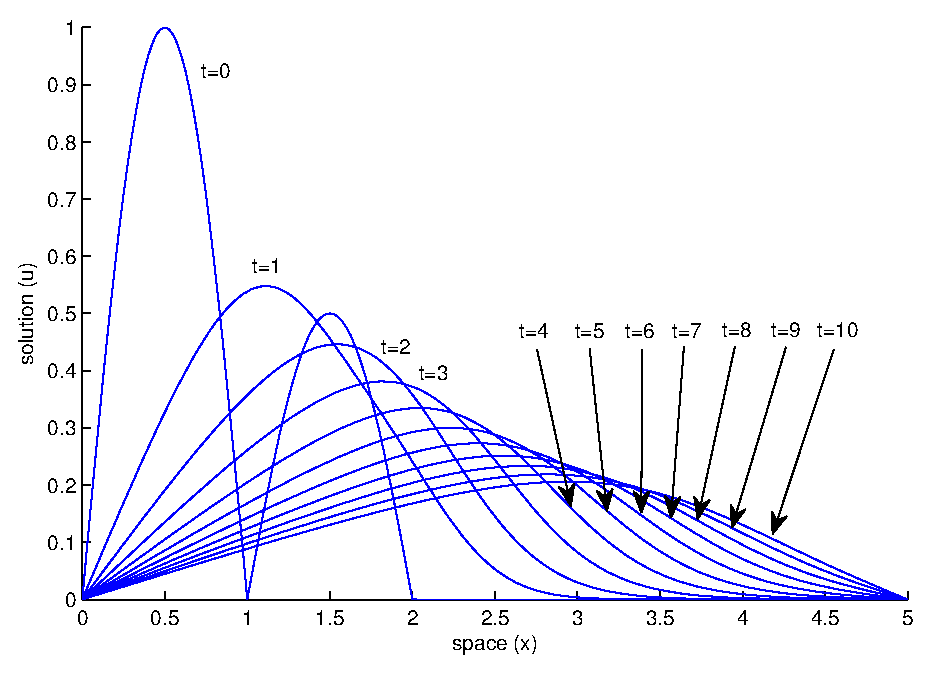
\includegraphics[width=0.50\textwidth]{example2epsilon01.eps}} %\hspace{0.5cm}
	\subfloat[]{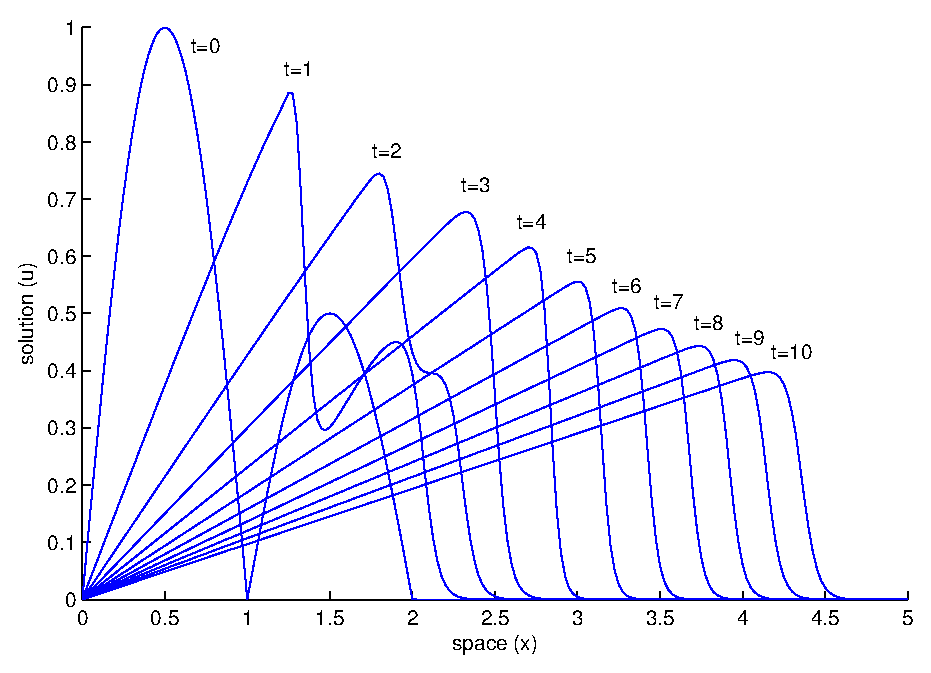
\includegraphics[width=0.50\textwidth]{example2epsilon001.eps}}
	\caption{Solución para distintos instantes y valores de $\varepsilon$, ambos con $n=m=200$ y $t_{max}=10$. (\textbf{a}) $\varepsilon =0.1$;  (\textbf{b}) $\varepsilon =0.01$.}
	\label{mittal}
\end{figure}

\vspace{-12pt}
\begin{table}[h!]
	\small
	\centering
	\begin{tabular}{cccc}
		\toprule
		\boldmath $x$   &\boldmath $t$  &\boldmath $\varepsilon =0.1$ &\boldmath $\varepsilon =0.01$ \\
		\midrule
		1.5 & 2  &  0.44533     &  0.63548                          \\
		& 4  &  0.28961     &  0.34573                          \\
		& 6  &  0.20701     &  0.23678                          \\
		& 8  &  0.16020     &  0.17999                          \\
		& 10 &  0.13041     &  0.14516                          \\
		\hline
		3   & 2  &  0.02972     &  0.00000                          \\
		& 4  &  0.14900     &  0.00470                          \\
		& 6  &  0.22312     &  0.47269                          \\
		& 8  &  0.22501     &  0.35971                          \\
		& 10 &  0.20562     &  0.29021                          \\
		\hline
		4.5 & 2  &  0.00001     &  0.00000                          \\
		& 4  &  0.00145     &  0.00000                          \\
		& 6  &  0.01171     &  0.00000                          \\
		& 8  &  0.03557     &  0.00000                          \\
		& 10 &  0.06242     &  0.02066                          \\
		\bottomrule
	\end{tabular}
	\caption{Resultados numéricos de la solución aproximada para distintos valores de $x, t$ y $\varepsilon$.}\label{example2table}
\end{table}

Estos resultados son muy similares a aquellos obtenidos por Mittal y Singhal en \cite{MS}, donde transforman la ecuación de Burgers en un sistema de ecuaciones diferenciales ordinarias no lineales y posteriormente lo resuelven mediante el método de segundo orden de Runge-Kutta-Chebyshev. Aunque las técnicas usadas para resolver el problema son diferentes, los resultados obtenidos por Mittal-Singhal y los nuestros, mostrados en la Tabla \ref{example2table} y en la Figura \ref{mittal}, son del mismo orden de magnitud. Como podemos ver en la Figura \ref{mittal}, ocurre efectivamente, que cuanto más pequeño es $\varepsilon$, más lenta es la atenuación. Aunque en este ejemplo hemos usado una condición inicial definida a trozos, y normalmente éstas siempre traen más problemas, nuestros resultados obtenidos han sido satisfactorios. Dado que hemos considerado un límite del tiempo de estudio bastante elevado ($t=10$), hemos tenido que coger un valor de $m$ más grande con el objetivo de mantener un buen tamaño de mallado. Los resultados mostrados tanto en la Figura \ref{mittal} como en la Tabla \ref{example2table} son los mismos tanto si usamos el método de Newton, como el de Traub o como el de M5.

\section{Conclusiones}

Como hemos visto en los Ejemplos 1 y 2, nuestro método tiene la misma precisión que aquellos métodos que aplican la transformación de Hopf-Cole o Runge-Kutta al sistema de ecuaciones diferenciales equivalente. Nuestro método es mucho más directo, dado que no requiere la aplicación de la mencionada transformación.

También hemos aprovechado los resultados numéricos para sacar algunas conclusiones acerca de la importancia de la cantidad de subintervalos en el espacio y en el tiempo para la obtención del mallado sobre el que calculamos la solución, así como la dependencia entre el error y el valor de la constante de Reynolds: si queremos reducir el error, podemos tomar más subintervalos en el espacio, aunque el coste computacional se incrementará debido a que entonces habrá más incógnitas a resolver por sistema. Otra forma de reducir el error es cogiendo más subintervalos en el tiempo, sin embargo hemos visto que hay un límite a partir del cual si seguimos cogiendo mayores valores de $m$, el error se incrementará de nuevo. Al mismo tiempo, tomar más subintervalos en el tiempo también significa incrementar el coste computacional, ya que entonces habrá más sistemas a resolver. También hemos visto que coger mayores valores de atenuación ($\varepsilon$) implica un mayor error debido a que como más rápida es la atenuación, más abrupta es la curva y peor es la aproximación; para solucionar esto, se deberían tomar más subintervalos en el tiempo, aunque no hay necesidad de tomar más subintervalos en el espacio.